\chapter{Robust and Sparse Supervised Learning}\label{ch:SL}
%
%
In this chapter we now focus on supervised learning as described in \cref{sec:PSL}. 
\cite{bungert2021clip, bungert2021neural, kabri2023resolution, bungert2022bregman}
%
\paragraph{Remark on Notation} In the following we deviate from the notation of the previous part. Most notably the input space is now denoted by $\Inp$ instead of $\domain$. Furthermore, we employ $\OutSpace$ to denote an abstract output space.
\section{Setting}
%
We are given a finite training set $\tset\subset\Inp\times\OutSpace$. For a family of functions $f_\param:\Inp\to\OutSpace$ parameterized by $\param\in \param$ we consider the empirical  minimization
%
\begin{align*}
\min_{\param\in\param} \empLoss(\param) 
\end{align*} 
%
where for a function $\ell:\OutSpace\times\OutSpace\to\R$ we define
\begin{align}\label{eq:empLoss}
\empLoss(\param)  := \frac{1}{\abs{\tset}}\sum_{(x,y)\in \tset} \ell(f_\param(x), y).
\end{align}
%
Assuming that $\tset$ is sampled from a joint distribution $\pi$ on $\Inp\times\OutSpace$ this approximates the infeasible population risk minimization
%
\begin{align*}
\int_{\Inp\times\OutSpace} \ell(f_\param(x), y) d\pi(x,y).
\end{align*}
%
In this thesis we focus on feed-forward neural networks, i.e., we consider layers of the form
%
\begin{align*}
\Phi(w, W, b)(z):= wz + \sigma(Wz + b)
\end{align*}
%
where $w\in\R$ models a residual connection, $W\in\R^{n\times n}$ is a weight matrix, $b\in\R^n$ a bias vector and $z\in\R^{m}$. We consider a concatenation of $L\in\N$ such layers, which then forms a neural network
%
\begin{align*}
f_\param = \Phi^L\circ\ldots\circ\Phi^1
\end{align*} 
%
with parameters $\param =(w_1,\ldots, w_L, W_1,\ldots, W_L, b_1,\ldots, b_L)\in\param$ and layers $\Phi^i := \Phi(w_i, W_i, b_i)$.
%
\paragraph{MLP}

\paragraph{Convolutions}\label{sec:convlayer}

\paragraph{ResNets}
%
\subsection{Gradient Computation and Stochastic Gradient Descent}\label{sec:SGD}
%
%
Training a neural network requires to solve a optimization problem w.r.t. to the parameters $\param\in\Param$. In this work we only focus on first order methods, however both zero \cite{Riedl} and second order methods \cite{Hessian} have been successfully applied in this context. Employing first order methods, requires to evaluate the gradient $\nabla_\theta \empLoss$, however in this scenario it is not common to compute the full gradient but rather to have a gradient estimator. This estimator is usually obtained by randomly dividing the train set $\trSet$ into disjoint minibatches $B_1\cup\ldots\cup B_b = \trSet$ and then successively computing the gradient of the minibatch loss
%
\begin{align*}
\frac{1}{\abs{B_i}}\sum_{(x,y)\in B_i} \ell(f_\param(x), y).
\end{align*}
%
Iterating over all batches $i=1,\ldots,b$ is referred to as one epoch. From a mathematical point of view this yields stochastic optimization methods, since in each step the true gradient is replaced by an estimator. In the abstract setting we let $(\Omega,F,\P)$ be a probability space and consider a function $g:\Param\times \Omega\to \Param$ as an unbiased estimator of $\nabla\empLoss$, i.e.
%
\begin{align*}
\Exp{g(\param;\omega)} = \nabla\empLoss(\param)\text{ for all } \param\in\Param.
\end{align*}
%
Most notably this method transforms the standard gradient descent update \cite{cauchy1847methode}
%
\begin{align*}
\param^{(k+1)} = \param^{(k)} - \tau^{(k)} \nabla \empLoss(\theta^{(k)})
\end{align*}
%
to \emph{stochastic} gradient descent \cite{robbins1951stochastic}
%
\begin{align*}
\text{draw }&\omega^{(k)}\text{ from }\Omega\text{ using the law of }\P,\\
g^{(k)} &:= {g(\param^{(k)};\omega^{(k)})},\\
\param^{(k+1)} &:= \param^{(k)} - \tau^{(k)} g^{(k)}.
\end{align*}
\section{Adversarial Stability}

%
\section{Sparsity via Bregman Iterations: \cite{bungert2022bregman}}

Intro sparsity blah blah
%
\begin{enumerate}
\item efficency
\item robustness
\item generalization
\end{enumerate}
%
\subsection{Preliminaries on Convex Analysis and Bregman Iterations}

We first review some necessary concepts from convex analysis that allow us to introduce the framework in \cite{bungert2022bregman}. We refer to \cite{benning2018modern, rockafellar1997convex, bauschke2011convex} for a more exhaustive introduction to the topics.
%
The functional $\func$ is called lower semicontinuous if $\func(u)\leq\liminf_{n\to\infty}\func(u_n)$ holds for all sequences $(u_n)_{n\in\N}\subset\Param$ converging to $u$.
%
\begin{definition}{}{}
Given a Hilbert space $\Param$ and a functional $\func:\Param\to(-\infty,\infty]$.
%
\begin{enumerate}
\item The functional $\func$ is called convex, if
%
\begin{align}
    \func(\lambda\overline{\param}+(1-\lambda)\param)\leq
    \lambda\func(\overline{\param})
    +(1-\lambda)\func(\param),\quad\forall\lambda\in[0,1],\,\overline{\param},\param\in\Param.
\end{align}
%
\item The effective domain of $\func$ is defined as $\dom(\func):=\{\param\in\Param\st\func(\param)\neq\infty\}$ and $\func$ is called proper if $\dom(\func)\neq\emptyset$.
\end{enumerate} 
\end{definition}
%
%
In the following we want to consider functionals $J$ that are convex, but not necessarily differentiable. Therefor, we define the subdifferential.
%
\begin{definition}{}{}
of a convex {and proper} functional $\func:\Param\to(-\infty,\infty]$ at a point $\param\in\Param$ as
% ---------------------------------------------------------
\begin{align}
\label{eq:subgrad}
    \partial\func(\param) := \left\lbrace \sg\in\Param \st \func(\param) + \langle\sg,\overline{\param}-\param \rangle \leq \func(\overline{\param}),\;\forall\overline{\param}\in\Param\right\rbrace.
\end{align}
\end{definition}
% ---------------------------------------------------------
If $\func$ is differentiable, then the subdifferntial coincides with the classical gradient (or Fr\'echet derivative). We denote $\dom(\partial\func):=\{\param\in\Param\st\partial\func(\param)\neq\emptyset\}$ and observe that $\dom(\partial\func)\subset\dom(\func)$.

The main algorithm in this section are so-called Bregman iterations, for which we first define the Bregman distance.
%
\begin{definition}{Bregman Distance}{}
Let $\func:\Param\to(-\infty,\infty]$ be a proper, convex functional. Then we define for $\param\in\dom(\partial\func),\overline{\param}\in\Param$
% ---------------------------------------------------------
\begin{align}\label{eq:bregman_distance}
D^\sg_\func(\overline{\param},\param) := \func(\overline \param)-\func({\param})-\langle\sg,\overline\param-{\param}\rangle,\quad\sg\in\partial\func(\param).
\end{align}
%
For $\sg\in\partial\func({\param})$ and $\overline\sg\in\partial\func(\overline{\param})$ we define the \emph{symmetric} Bregman distance as
\begin{align}
D^\mathrm{sym}_\func(\overline{\param},\param) := D^\sg_\func(\overline{\param},\param) + D^{\overline{\sg}}_\func(\param,\overline\param).
\end{align}
\end{definition}
% ---------------------------------------------------------
Intuitively, the Bregman distance $D^\sg_\func(\overline{\param},\param)$, measures the distance of $\func$ to its linearization around $\param$, see \cref{fig:Bregdist}. If $J$ is differentiable, then the subdifferential is single valued---we can suppress the sup script $\sg$---and we have
%
\begin{align*}
D_J(\overline\param,\param) = \func(\overline \param)-\func({\param})-\langle\,\nabla \func(\param), \overline\param-{\param}\rangle.
\end{align*}
%
\begin{figure}
\centering
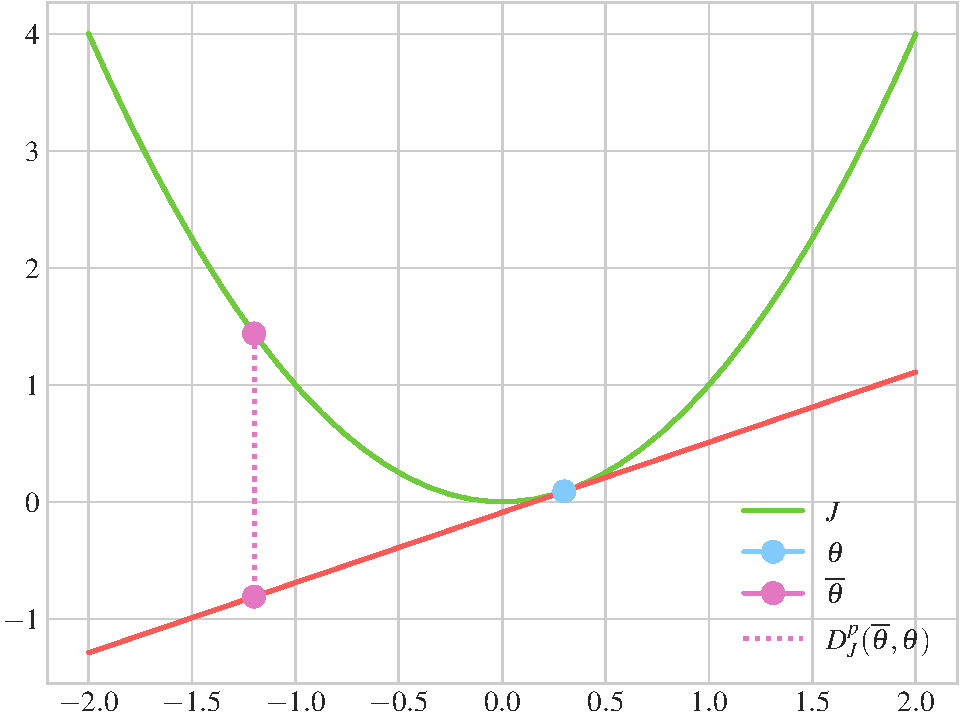
\includegraphics[width=.7\textwidth]{code/Bregman/lin_dist.pdf}
\caption{Visualization of the Bregman distance.}\label{fig:Bregdist}
\end{figure}
%
\begin{example}{}{ex:BregNorm}
For $\Param=\R^n$ and $J=\frac{1}{2}\norm{\cdot}_2^2$ we see that $\partial J(\param) = \{\param\}$ and therefore
%
\begin{align*}
D_J^p(\overline{\param}, \param) &= 
\frac{1}{2}\langle \overline\param,\overline\param\rangle - 
\frac{1}{2}\langle \param,\param\rangle - \langle \param, \overline\param-\param\rangle 
\\&=
\frac{1}{2}\langle \overline\param,\overline\param\rangle+
\frac{1}{2}\langle \param,\param\rangle -
\langle \param,\overline\param\rangle
\\&=
\frac{1}{2}\norm{\overline\param - \param}_2^2 = J(\overline\param - \param).
\end{align*}
\end{example}
%
We can easily see that in general it is neither definite, symmetric nor fulfills the triangle inequality, hence it is not a metric. 
However, it fulfills the two distance axioms
\begin{align}
D^\sg_\func(\overline{\param},\param) \geq 0,\quad D^\sg_\func(\param,\param)=0,\quad\forall\overline{\param}\in\Param,\param\in\dom(\partial\func).
\end{align}
%
The same holds for the symmetric Bregman distance, where additionally---as the name suggests---the symmetry property is fulfilled.
%
%
The last concept that is crucial in \cite{bungert2022bregman} is the so-called proximal operator.
%
\begin{definition}{}{}
Let $\func:\Param\to(-\infty,\infty]$  be convex, proper and lower semicontinuous functional, then we define the \emph{proximal operator} as
\begin{align*}
    \prox{\func}(\overline{\param}) := \argmin_{\param\in\Param} \frac{1}{2}\norm{\param-\overline{\param}}^2 + \func(\param).
\end{align*}
\end{definition}
%
If $\func$ is additionally a closed function, i.e., its sublevel sets
%
\begin{align*}
N_\alpha = \{\param\in\dom \func: \func(\param)\leq \param\}
\end{align*} 
%
are closed for every $\alpha\in\R$ then we have that the function $\tilde J = \frac{1}{2}\norm{\param -\cdot}^2 + \func(\param)$ is closed, proper and \emph{strongly} convex and therefore has a unique minimizer, see \cite[Thm. 27.1]{rockafellar1997convex}.
%
\begin{example}{}{}
If $\func=\norm\cdot$ is a norm and $\lambda>0$ then we have that (see e.g. \cite{parikh2014proximal})
%
\begin{align*}
\prox{\lambda\func}(\pparam) = 
\pparam - \operatorname{Proj}_{\norm{\cdot}^\ast}(\pparam/\lambda)
\end{align*}
%
where $\operatorname{Proj}_{\norm{\cdot}^\ast}$ denotes the projection operator w.r.t. the dual norm $\norm{\param}^\ast = \sup\{\abs{\langle f , \param\rangle}: f\in\Theta^\ast\}$. In the case of $\ell^p$ norms on $\R^n$ we know that that 
%
\begin{align*}
\norm{\param}_p^\ast = \norm{\param}_q
\end{align*}
%
with $1/p + 1/q = 1$ with the notational convention of $1/\infty=0$. Especially relevant are the cases $p\in\{1,2\}$. Here, we then have that
%
\begin{align*}
\prox{\lambda\norm{\cdot}_2}(\pparam) = 
%
\pparam\,\left(1 - \min\left\{\frac{\lambda}{\norm{\pparam}_2}, 1\right\}\right)=
%
\begin{cases}
\pparam\,(1 - \lambda/\norm{\pparam}_2) &\text{ if } \norm{\pparam}_2 \geq \lambda\\
0 &\text{ else}
\end{cases}
\end{align*}
%
and for $i=1,\ldots,n$
%
\begin{align*}
\prox{\lambda\norm{\cdot}_1}(\pparam)_i
%
= \sign(\pparam_i)\, \max\left\{\abs{\pparam_i} - \lambda, 0\right\} =
%
\begin{cases}
\pparam_i -\lambda &\text{ if }\pparam > \lambda\\
0 &\text{ if } \abs{\pparam_i}\leq \lambda\\
\pparam_i +\lambda &\text{ if }\pparam < -\lambda
\end{cases}
\end{align*}
%
the so called \emph{soft thresholding operator}. 
\end{example}
%
%
\begin{example}{Group Norms}{}
Another relevant functional $\func$ is the group norm $\ell_{1,2}$ that---in the context of sparse neural networks---was first employed by \cite{scardapane2017group}. Here, we assume that the parameters in $\Theta$ can be grouped in a collection of parameters $\mathcal{G}$, for which we the choose
%
\begin{align*}
\func(\param) = \sum_{g\in\mathcal{G}} \sqrt{\# \mathcal{G}} \norm{g}_2
\end{align*}
%
In this case the proximal operator is given as
%
\begin{align*}
\prox{\lambda\func}(\pparam)_g = g \, 
\max\left\{1- \min\left\{
\frac{\lambda\,\sqrt{\# \mathcal{G}}}{\norm{g}_2}
,1 \right\}
,0\right\}
\end{align*}
\end{example}
%
%
%\begin{example}{Elastic Net}{}
%For a convex functional $\func$ we also consider the elastic net version $J_\delta = J + \frac{1}{2\delta}\norm{\cdot}^2$ in the following. Here we see that 
%%
%\begin{align*}
%\prox{\lambda\func_\delta}(\pparam) &= \argmin_{\param\in\Param} \frac{1}{2}\norm{\param-\overline{\param}}^2 + \lambda\func(\param) + \frac{1}{2\delta}\norm{\param}^2\\ 
%%
%&= 
%\argmin_{\param\in\Param} \frac{1+\delta}{2\delta} \norm{\param}^2 - \frac{1}{2}\langle \param,\pparam\rangle + \lambda\func(\param)\\
%%
%&= \argmin_{\param\in\Param} \frac{1}{2} \norm{\param}^2 - \frac{1}{2}
%\left\langle \param,\frac{\delta}{1+\delta}\, \pparam\right\rangle + (1 + \delta)^{-1}\lambda J(\param)\\
%&= 
%\prox{\frac{\delta}{1+\delta}\lambda \func}\left(\frac{\delta}{1+\delta}\, \pparam\right).
%\end{align*}
%%
%Setting $\tilde\delta = \delta(1+\delta)^{-1}$ we see that for $\func = \norm{\cdot}_1$ we have that
%%
%\begin{align*}
%\prox{\lambda\func_\delta}(\pparam)_i = \sign(\tilde\delta\, \pparam_i) 
%\max\left\{
%\abs{\tilde\delta\,  \pparam_i} - \lambda, 0
%\right\}
%=
%\sign(\pparam_i)
%\end{align*}
%\end{example}
%
The the optimality conditions yield for $\param=\prox{J}(\overline\param)$ 
%
\begin{align*}
\param - \overline\param \in \partial \func(\param).
%
\end{align*}
%
If $J$ is differentiable, we then have
%
\begin{align*}
\param - \nabla J(\param) = \overline\param\Leftrightarrow
\theta = (I + \nabla J)^{-1}(\overline\theta).
\end{align*}\todo{check this!}
%
%
%
We first consider the following implicit Euler scheme\todo{Minimizing Movment proximal point}, for a step size $\tau>0$
\begin{subequations}\label{eq:bregman_iteration}
\begin{align}
    \param^{(k+1)} &= \argmin_{\param\in\Param} D^{\sg^{(k)}}_\func\left(\param,\param^{(k)}\right) + \tau^{}\empLoss(\param), \\
    \sg^{(k+1)} &= \sg^{(k)} - \tau^{}\nabla\empLoss(\param^{(k+1)}) \in \partial \func(\param^{(k+1)})
\end{align}
\end{subequations}
%
which is known as the \emph{Bregman iteration} \cite{osher2005iterative}. The intuitive interpretation here is, that in each step we want to minimize $\empLoss$ while also being close to the previous iterate in terms of the Bregman distance induced by $J$. Therefore, the very nature of Bregman iterations means starting with a iterate $\param^{(0)}$ that has a low value in $J$---preferably $J(\param^{(0)}) = 0$---and only increase $J(\param^{(k)})$ gradually as $k$ increases.
%
\begin{remark}{}{}
Originally, the iterations were employed for solving inverse problems. Here, we are given a forward operator $A:\Param\to\tilde{\Param}$ and a noisy measurement $f= A\param +\delta$ where $\delta\in \tilde{\Param}$ is additive noise. The loss function is then of the form
%
\begin{align*}
\empLoss = \frac{1}{2}\norm{A\cdot - f}^2_2
\end{align*}
%
for which one can show that the Bregman iterations converge to a solution of
%
\begin{align}\label{eq:Bregexact}
\min \left\{\func(\param): A\theta = f\right\},
\end{align}
%
see e.g. \cite{osher2005iterative}. In comparison the concept of adding a regularizing term with parameter $\lambda>0$, i.e. considering the problem
%
\begin{align*}
\min_\param \empLoss(\param) + \lambda J(\param) 
\end{align*}
%
actually modifies the minimizers. In this sense Bregman iterations do not introduce a bias.
\end{remark}
%
%
\begin{example}{}{ex:BregCat}
In order to get an intuition about the behavior of Bregman iterations, we consider an image denoising task. I.e. we are given a noisy image $\R^{n\times m}\ni f = u + \delta$ where $\delta\in\R^{n\times m}$ is additive noise. In order to obtain $u\in\R^{n\times n}$ from $f$ we employ the TV functional 
%
\begin{align*}
J(u) = TV(u) := MISSING,
\end{align*}
%
together with the loss function $\empLoss(u):= \frac{1}{2}\norm{u-f}^2_2$.
%
We start with an image $u^{(0)}$ such that $TV(u^{(0)})=0$, i.e. a constant image. In \cref{fig:BregCat} we visualize the iteration. At lower iterations $u^{(k)}$ only displays features on a larger scale, while at the end, the iteration converges back to smallest possible scale, the noisy data. In order to obtain an appropriate denoising, one needs to employ a early stopping here. This fits well to the insight from \cref{eq:Bregexact} since here the forward operator is the identity. I.e.
%
\begin{align*}
\{ u: \frac{1}{2}\norm{u-f}^2=0\} = \{f\}. 
\end{align*}
%
It should also be noted that this example only serves a explanatory purpose. In practice directly applying \cref{eq:bregman_iteration} for $J=TV$ can become infeasible since the first minimization problem is expensive.
\end{example}
%
%
%
%
\begin{figure}
\begin{minipage}{\textwidth}%
\begin{subfigure}{.3\textwidth}%
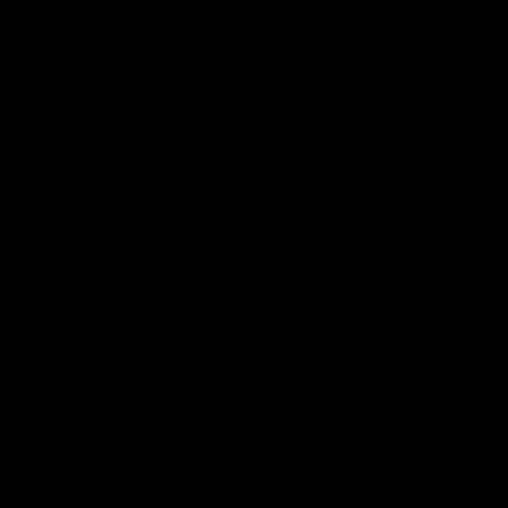
\includegraphics[width=\textwidth]{atelier/breg_cat/cat-0.png}
\subcaption{Iteration $k=0$}
\end{subfigure}\hfill%
\begin{subfigure}{.3\textwidth}%
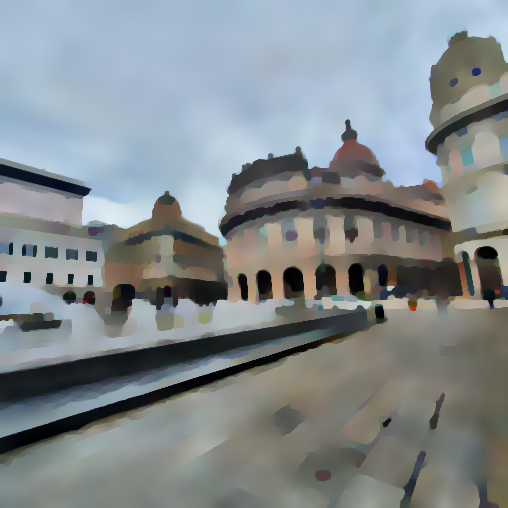
\includegraphics[width=\textwidth]{atelier/breg_cat/cat-10.png}
\subcaption{Iteration $k=10$}
\end{subfigure}\hfill%
\begin{subfigure}{.3\textwidth}%
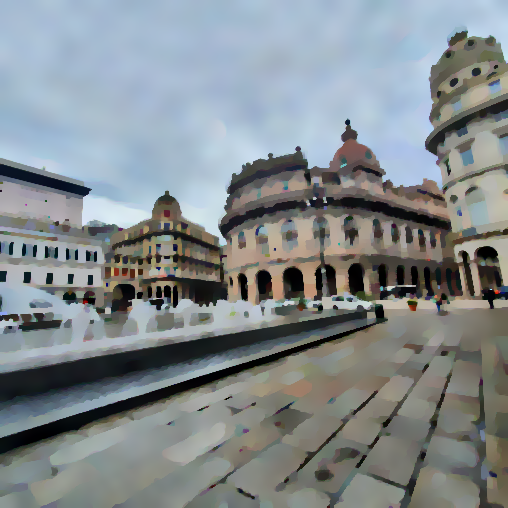
\includegraphics[width=\textwidth]{atelier/breg_cat/cat-20.png}
\subcaption{Iteration $k=20$}%
\end{subfigure}
\end{minipage}\\%

\begin{minipage}{\textwidth}%
\begin{subfigure}{.3\textwidth}%
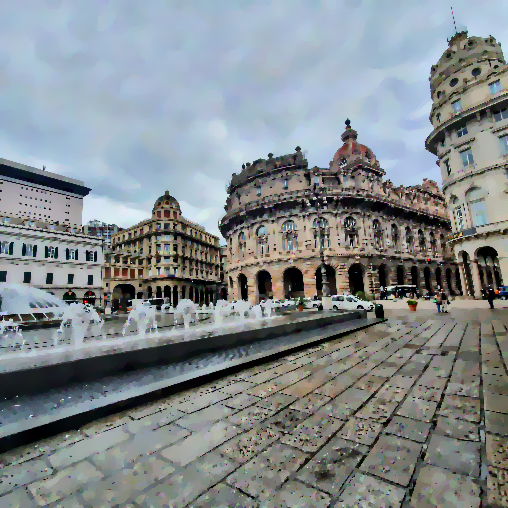
\includegraphics[width=\textwidth]{atelier/breg_cat/cat-50.png}%
\subcaption{Iteration $k=50$}%
\end{subfigure}\hfill%
\begin{subfigure}{.3\textwidth}%
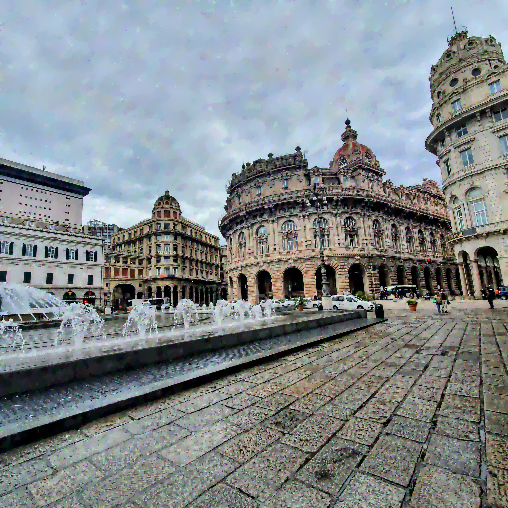
\includegraphics[width=\textwidth]{atelier/breg_cat/cat-95.png}%
\subcaption{Iteration $k=100$}%
\end{subfigure}\hfill%
\begin{subfigure}{.3\textwidth}%
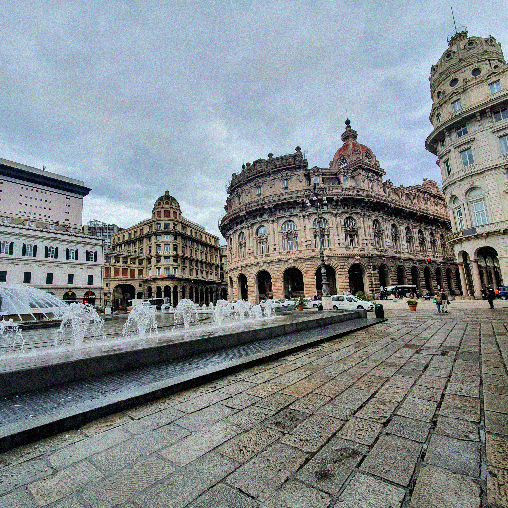
\includegraphics[width=\textwidth]{atelier/breg_cat/data.png}
\subcaption{Iteration $k=500$}
\end{subfigure}%
\end{minipage}%
%
\caption{Bregman iterations for image denoising in \cref{ex:BregCat}}\label{fig:BregCat}
\end{figure}


If $J=\frac{1}{2}\norm{\cdot}_2^2$ as in \cref{ex:BregNorm} then this amounts to the step
%
\begin{align*}
\param^{(k+1)} &= \argmin_{\param\in\Param} \frac{1}{2}\norm{\param - \param^{(k)}}^2_2 + \tau^{}\empLoss(\param),
\end{align*}
%
where the optimality conditions then yield
%
\begin{align*}
\param^{(k+1)} - \param^{(k)} + \tau \nabla \empLoss(\param^{(k+1)}) = 0
\Leftrightarrow \param^{(k+1)}= \param^{(k)} - \tau \nabla \empLoss(\param^{(k+1)})
\end{align*}
%
which is a standard implicit Euler iteration. The time continuous flow for $\tau\to 0$ is known as the \emph{inverse scale space} flow \cite{burger2006nonlinear,burger2007inverse},
%
\begin{align*}
\begin{cases}
    \dot{\sg}_t = - \nabla\empLoss(\param_t), \\
    \sg_t \in \partial \func(\param_t),
\end{cases}
\end{align*}
%
where again for $J=\frac{1}{2}\norm{\cdot}_2^2$ we obtain that $\partial J(\param_t) = \param_t$ and therefore obtain the standard gradient flow. Hence we see, that the inverse scale space flow is a generalization of the standard gradient flow. 
%
%
%
\subsection{Linearized Bregman Iterations and Mirror Descent}
%
The minimization step in \cref{eq:bregman_iteration} is infeasible for large scale applications, especially in our setting of neural networks. Therefore, we employ the idea introduced in \cite{yin2008bregman, cai2009convergence}. Here, we first linearize the loss function around the previous iterate,
%
\begin{align*}
\empLoss(\param) \approx \empLoss(\param^{(k)}) + 
\left\langle \nabla\empLoss(\param^{(k)}), \param - \param^{(k)}
\right\rangle.
\end{align*} 
%
The next step is to replace $\func$ with the strongly convex elastic net regularization%
\begin{align}\label{eq:elastic_net}
\func_\delta:= \func + \frac{1}{2\delta}\norm{\cdot}^2_2.
\end{align}
%
The minimization step then transforms to
%
\begin{align}\label{eq:LinBregDer}
\argmin_{\param\in\Param} &D^{\sg^{(k)}}_{\func_\delta} \left(\param,\param^{(k)}\right) + \tau^{}\left\langle \nabla\empLoss(\param^{(k)}), \param
\right\rangle\\&= 
\argmin_{\param\in\Param}
J(\param) + \frac{1}{2\delta} \norm{\param}^{2}_2 - 
\langle \sg^{k}, \param\rangle +
\tau^{}\left\langle \nabla\empLoss(\param^{(k)}), \param
\right\rangle\nonumber\\
&=
\argmin_{\param\in\Param}
J(\param) + \frac{1}{2\delta} \norm{\param - \delta(\sg^{(k)} -\tau \nabla\empLoss(\param^{(k)})}^2_2 - \underbrace{\norm{\sg^{(k)} -\tau \nabla\empLoss(\param^{(k)})}^2_2}_{\text{constant in } \param}\nonumber\\
&=
\prox{\delta \func}\left(\delta\left(\sg^{(k)} -\tau \nabla\empLoss(\param^{(k)}\right)\right).\nonumber%
\end{align}
%
Note that here $\sg^{(k)}$ is a subgradient of $J_\delta$ at $\param$ therefore we derive the subgradient update rule
%
\begin{align*}
\sg^{(k+1)} := \sg^{(k)} - \tau \empLoss(\param^{(k)}).
\end{align*}
%
This finally yields the linearized Bregman iterations
%
\begin{subequations}\label{eq:lin_bregman_iteration}
\begin{align}
\sg^{(k+1)} = \sg^{(k)} - \tau \nabla\empLoss(\param^{(k)}),\\
\param^{(k+1)} = \prox{\delta J}(\delta \sg^{(k+1)}).
\end{align}
\end{subequations}
%
%
The last line is equivalent to $\sg^{(k+1)}\in\partial J_\delta(\param^{(k+1)})$ for which we obtain the continuous linearized flow
%
\begin{align*}
\dot{\sg}_t &= -\nabla \empLoss(\param_t),\\
\sg_t &\in \partial J_\delta(\param_t).
\end{align*}\todo{A lot of citations missing here}
%
%
As already noticed by \cite{??} linearized Bregman iteration are equivalent to mirror descent in some situations. We show the equivalence in the following, where we employ similar arguments as in \cite{Duchi}.
%
One assumes to be given a differentiable and strongly convex function $h:\Param\to\R$, i.e.,
%
\begin{align*}
h(\overline\param) - h(\param) - \langle\nabla h(\param), \overline\param - \param \rangle \geq  
\frac{1}{2} \norm{\overline\param - \param}^2_2
\end{align*}
%
for all $\param,\overline\param\in\Param$. The mirror descent update then reads (\cite{nemirovskij1983problem, beck2003mirror})
%
\begin{align}\label{eq:mirror}
\theta^{(k+1)} = \nabla h^\ast\left(\nabla h\left(\theta^{(k)}\right) - \tau \empLoss(\param^{(k)})\right)
\end{align}
%
where $h^\ast$ denotes the Fenchel conjugate
%
\begin{align*}
h^\ast(\sg) = \sup_{\param} \langle \sg, \param\rangle - h(\param)
\end{align*}
%
with the gradient
%
\begin{align*}
\nabla h^\ast(\sg) = \argmax_{\param} \left\{ \langle\sg, \param\rangle - h(\param)\rangle\right\}.
\end{align*}
%
Therefore, we see that \cref{eq:mirror} can be written as
%
\begin{align*}
\param^{(k+1)} &= \argmax_\param
\left\{\left\langle\nabla h\left(\theta^{(k)}\right) - \tau \empLoss(\param^{(k)}), \param \right\rangle - h(\param)\right\}\\
&=
\argmax_\param \left\{-D_h(\param, \param^{(k)})-\tau\left\langle \empLoss(\param^{(k)}), \param \right\rangle\right\}\\
&=
\argmin_\param \left\{D_h(\param, \param^{(k)})+\tau\left\langle \empLoss(\param^{(k)}), \param \right\rangle\right\}
\end{align*}
%
which was our starting point to derive linearized Bregman iterations for $h=\func_{\delta}$ in \cref{eq:LinBregDer}. In fact, we can always find a convex functional $\func:\Theta\to\R$ such that $h = J + \frac{1}{2}\norm{\cdot}_2^2$ for which we see, that \cref{eq:lin_bregman_iteration} is a more general formulation of \cref{eq:mirror}.
%
%
\subsection{Stochastic and Momentum Variants}\label{sec:Bregmom}
%
%
We want to employ linearized Bregman iterations to train a neural network. As mentioned in \cref{sec:SGD} we therefore do not compute the full gradient of $\empLoss$ but rather a minibatched variant. This yields stochastic Bregman Iterations
%

\begin{align}\label{eq:stochlinbreg}
\begin{split}
\text{draw }&\omega^{(k)}\text{ from }\Omega\text{ using the law of }\P,\\
g^{(k)} &:= {g(\param^{(k)};\omega^{(k)})},\\
v^{(k+1)} &:= v^{(k)} - \tau^{(k)} g^{(k)},\\
\param^{(k+1)} &:= \prox{\delta J}(\delta v^{(k+1)}).
\end{split}
\end{align}
%
The basic update scheme is given as the linearized Bregman iterations from\cite{osher2005iterative}, however the presence of a stochastic gradient estimator significantly complicates the convergence analysis, as observed in \cref{sec:ConvAna}. However, this algorithm can now be efficiently employed to train a neural network. For the analogous stochastic mirror descent algorithm we refer to \cite{nemirovski2009robust}.
%
\paragraph{Momentum Variant} Typically, the learning process of a neural network can be improved by introducing a momentum term (see e.g. \cite{nesterov1983method, qian1999momentum}) in the optimizer. In our case this can be achieved, by replacing the gradient update on the subgradient variable. In \cite{bungert2022bregman} we first consider the inertia version of the gradient flow as
%
\begin{align*}
\begin{cases}
    \gamma \ddot{v}_t + \dot{v}_t = -\nabla\empLoss(\param_t), \\
    v_t \in \partial \func_\delta(\param_t).
\end{cases}
\end{align*}
%
for which the discretization then reads
%
\begin{align}\label{eq:momBreg}
\begin{split}
m^{(k+1)} &= \beta^{(k)} m^{(k)} + (1-\beta^{(k)})\tau^{(k)} g^{(k)},\\
v^{(k+1)} &= v^{(k)} - m^{(k+1)},\\
\param^{(k+1)} &= \prox{\delta\func}(\delta v^{(k+1)}).
\end{split}
\end{align}
%
%
\paragraph{Adamized Bregman Iteration} We shortly remark that one can replace the momentum update in \cref{eq:momBreg} with a Adam update \cite{kingma2014adam}. This then yields an Adamized version of linearized Bregman iterations as employed in \cite{bungert2022bregman}.


\subsection{Convergence of Stochastic Bregman Iterations}\label{sec:ConvAna}
%
%
While various previous works prove convergence of linearized Bregman iterations (see e.g. \cite{osher2005iterative, cai2009convergence}), the stochastic setting requires special treatment. In \cite{bungert2022bregman} the first guarantees for the algorithm in \cref{eq:stochlinbreg} were proven. Other work on convergence of stochastic Bregman iterations \cite{dragomir2021fast, hanzely2021fastest, zhang2018convergence, d2021stochastic} requires a differentiable functional $\func$. However, since our main motivation is to a functional in the flavor of the $\ell^1$ norm this is not applicable. Therefore, we present the novel convergence analysis of \cite{bungert2022bregman}.
%
%
\paragraph{Assumptions on the Gradient Estimator}
%
In order to obtain convergence guarantees, we need to assume mainly two properties on the gradient estimator $g(\cdot,\cdot)$. First we assume unbiasedness, which means
%
\begin{align*}
\Exp{g(\param;\omega)} = \nabla\empLoss(\param)\text{ for all }\param\in\Param.
\end{align*}
%
The second assumption we need in the following is referred to as \emph{bounded variance} of the estimator.
%
\begin{assumption}{Bounded variance}{ass:variance}
There exists a constant $\sigma>0$ such that for any $\param\in\Param$ it holds
\begin{align}
    \E\left[\norm{g(\param;\omega)-\nabla\empLoss(\param)}^2\right] \leq \sigma^2.
\end{align}
\end{assumption}
%
%
\begin{remark}{}{}
We want to remark, that this property is weaker than the bounded gradient assumption
%
\begin{align*}
\E\left[\norm{g(\param;\omega)}^2\right] \leq C
\end{align*}
%
for some constant $C>0$. In fact this condition can not be enforced together with a strong convexity assumption---which we employ in \cref{thm:??}---as shown in \cite{pmlr-v80-nguyen18c}.
\end{remark}
\paragraph{Assumptions on the Regularizer and on the Loss Function}
%
The assumptions on the regularization functional $\func$ are mild and merely ensure the well-definedness of the proximal mapping,
%
%
\begin{assumption}{Regularizer}{ass:regularizer}
We assume that $\func:\Param\to(-\infty,\infty]$ is a convex, proper, and lower semicontinuous functional on the Hilbert space $\Param$.
\end{assumption}
%
%
Our assumptions on the loss function $\empLoss$ are more restrictive. We require it to be bounded from below and differentiable, which are both standard assumptions. Additionally, we require Lipschitz continuity of the gradient, which also commonly employed in optimization literature.
%
\begin{assumption}{Loss function}{ass:loss}
We assume the following conditions on the loss function:
\begin{itemize}
    \item The loss function $\empLoss$ is bounded from below and without loss of generality we assume $\empLoss\geq 0$.
    \item The function $\empLoss$ is continuously differentiable.
    \item The gradient of the loss function $\param\mapsto\nabla\empLoss(\param)$ is $L$-Lipschitz for $L\in(0,\infty)$:
    \begin{align}\label{ineq:gradLip}
        \norm{\nabla\empLoss(\tilde\param)-\nabla\empLoss(\param)}\leq L \norm{\tilde\param-\param},\quad \forall \param,\tilde\param\in\Param.
    \end{align}
\end{itemize}
\end{assumption}
%
%
If the loss function $\empLoss$ fulfills the previous assumptions we are able to prove loss decay of the iterates in \cref{thm:decreasingloss}. However, in order to show convergence of the iterates we additionally need a convexity assumption. For a differentiable functional $J$, the authors in \cite{dragomir2021fast} assumed
%
\begin{align*}
\nu\ D_J(\pparam,\param) \leq D_\empLoss(\pparam,\param)
\end{align*}
%
which for twice differentiable $\func,\empLoss$ transfers to
%
\begin{align*}
\nu\ \nabla^2 \func \lesssim \nabla^2 \empLoss,\qquad\forall\pparam,\param\in\Param.
\end{align*}
%
Plugging in the definition of the Bregman dist $D_\empLoss$ we obtain
%
\begin{align*}
\nu\ D_J(\pparam,\param) \leq \empLoss(\pparam) - \empLoss(\param) - 
\langle \nabla\empLoss(\param), \pparam-\param\rangle.
\end{align*}
%
In this form one observes that this is in fact a convexity assumption on $\empLoss$ in a $\func$ dependent distance, as employed in \cite{bungert2022bregman}.
%
%
\begin{assumption}{Strong convexity}{ass:muconvex} 
For a proper convex function $H:\Param\to\R$ and $\nu\in(0,\infty)$, we say that the loss function $\param\mapsto\empLoss(\param)$ is $\nu$-strongly convex w.r.t. $H$, if
\begin{align}
\empLoss(\pparam) \geq \empLoss(\param) + \langle\nabla\empLoss(\param), \pparam - \param\rangle + \nu D_\func^\sg(\pparam,\param),\quad\forall\param,\pparam\in\Param, \sg\in\partial H(\param).
\end{align}
\end{assumption}
%
%
\begin{remark}{}{}
We have two relevant cases for the choice of $H$. For $H=\frac{1}{2}\norm{\cdot}^2$ \cref{ass:muconvex} reduces to standard strong $\nu$-convexity. The other relevant case, is $H=J_\delta$, i.e. we consider convexity w.r.t. to the functional $J_\delta$.
\end{remark}
%
%
\begin{remark}{}{}
In the setting of training a neural network, where we employ the empirical loss \cref{eq:empLoss}, this convexity assumption usually fails. While it is possible to enforce this conditions only locally around the minimum, this does not significantly improve the applicability. For future work, it would be desirable to enforce a  Kurdyka--\L ojasiewicz inequality, as in \cite{benning2018choose} for the deterministic case. 
\end{remark}

\paragraph{Loss Decay}
The first convergence result considers the loss decay of the iterates. Here, we do not assume convexity of the loss function. Under this assumptions \cite{benning2018choose, benning2018modern} were able to show the inequality
%
\begin{align*}
\begin{split}
\E\left[\empLoss(\param^{(k+1)})\right] + \frac{1}{\tau^{(k)}}\E\left[ D^\mathrm{sym}_\func(\param^{(k+1)},\param^{(k)})\right] + \frac{C}{2\delta\tau^{(k)}}\E\left[\norm{\param^{(k+1)}-\param^{(k)}}^2\right] \\
\leq \E\left[\empLoss(\param^{(k)})\right].
\end{split}
\end{align*}
%
%
In our setting, employing a stochastic gradient estimator, we are able to prove a similar estimate. Here, we obtain an additional term scaled $\sigma$ which controls the expected squared difference between the gradient estimator and the actual gradient. It should however be noted, that the proof is not only a trivial extension.
%
%
\begin{theorem}{\cite[Th. 2]{bungert2022bregman}: Loss decay}{thm:decreasingloss}
Assume that \cref{ass:loss,ass:variance,ass:regularizer} hold true, let $\delta>0$, and let the step sizes satisfy $\tau^{(k)} \leq \frac{2}{\delta L}$.
Then there exist constants $c,C>0$ such that for every $k\in\N$ the iterates of \labelcref{eq:stochlinbreg} satisfy 
\begin{align}\label{ineq:loss_decay}
    \begin{split}
    \E\left[\empLoss(\param^{(k+1)})\right] + \frac{1}{\tau^{(k)}}\E\left[ D^\mathrm{sym}_\func(\param^{(k+1)},\param^{(k)})\right] + \frac{C}{2\delta\tau^{(k)}}\E\left[\norm{\param^{(k+1)}-\param^{(k)}}^2\right] \\
    \leq \E\left[\empLoss(\param^{(k)})\right] + \tau^{(k)}\delta\frac{\sigma^2}{2c},
    \end{split}
\end{align}
\end{theorem}

\paragraph{Convergence of the Iterates}
Here, we have two cases respectively proving convergence w.r.t. the $L^2$ distance and the Bregman distance of $J_delta$. The first assumes strong convexity with $H=\frac{1}{2}\norm{\cdot}^2$ in \cref{ass:muconvex}.
%
%
\begin{theorem}{\cite[Th. 6]{bungert2022bregman}: Convergence in norm}{thm:cvgc_norm}
Assume that \cref{ass:loss,ass:variance,ass:regularizer} and \cref{ass:muconvex} for $H=\frac{1}{2}\norm{\cdot}^2$ hold true and let $\delta>0$.
Furthermore, assume that the step sizes $\tau^{(k)}$ are such that for all $k\in\N$:
\begin{align*}
    {\tau^{(k)}\leq \frac{\mu}{2\delta L^2}},\qquad
    \tau^{(k+1)} \leq \tau^{(k)}, \qquad
    \sum_{k=0}^\infty (\tau^{(k)})^2 < \infty, \qquad
    \sum_{k=0}^\infty \tau^{(k)} = \infty.
\end{align*}
The function $\mathcal{L}$ has a unique minimizer $\param^*$ and if $J(\param^*)<\infty$ the stochastic linearized Bregman iterations \labelcref{eq:stochlinbreg} satisfy the following:
\begin{itemize}
    \item Letting $d_k:=\E\left[D_{\func_\delta}^{v^{(k)}}(\param^*,\param^{(k)})\right]$ it holds
    \begin{align}\label{ineq:decay_bregman_distance}
        d_{k+1} - d_k + \frac{\mu}{4}\tau^{(k)}\E\left[\norm{\param^*-\param^{(k+1)}}^2\right]
        \leq  \frac{\sigma}{2}\left((\tau^{(k)})^2 +\Exp{\norm{\param^{(k)} - \param^{(k+1)}}^2}\right).
    \end{align}
    \item The iterates possess a subsequence converging in the $L^2$-sense of random variables: 
    \begin{align}
        \lim_{j\to\infty}\E\left[\norm{\param^*-\param^{(k_j)}}^2\right] = 0.
    \end{align}
\end{itemize}
{Here, $\func_\delta$ is defined as in \labelcref{eq:elastic_net}.}
\end{theorem}
%
%
For the second result we assume convexity w.r.t. the Bregman distance, i.e. we choose $H=\func_{\delta}$ in \cref{ass:muconvex}. This induces a relation between the Bregman distance of $\func$ and the loss function $\empLoss$, which has been similarly employed in \cite{dragomir2021fast}.
%
%
\begin{theorem}{\cite[Th. 11]{bungert2022bregman}: Convergence in the Bregman distance}{thm:cvgc_breg_dist}
Assume that \cref{ass:loss,ass:variance,ass:regularizer} and \cref{ass:muconvex} for $H=J_\delta$ hold true and let $\delta>0$.
The function $\mathcal{L}$ has a unique {minimizer} $\param^*$ and if $\func(\param^*)<\infty$ the stochastic linearized Bregman iterations \labelcref{eq:stochlinbreg} satisfy the following:
\begin{itemize}
    \item {Letting $d_k :=\E\left[D_{J_\delta}^{v^{(k)}}(\param^*,\param^{(k)})\right]$ it holds
    \begin{align}\label{eq:estimate_expects}
        % d_{k+1} \leq \left(1 - \tau^{(k)}\nu\right)d_k + (\tau^{(k)})^2\delta B.
        d_{k+1} \leq \left[1 - \tau^{(k)}\nu\left(1-\tau^{(k)}\frac{2\delta^2 L^2}{\nu}\right)\right]d_k + \delta(\tau^{(k)})^2\sigma^2.
    \end{align}}
    \item For any $\eps>0$ there exists $\tau>0$ such that if $\tau^{(k)}=\tau$ for all $k\in\N$ then
    \begin{align}
        \limsup_{k\to\infty} d_k \leq \eps.
    \end{align}
    \item If $\tau^{(k)}$ is such that
    \begin{align}\label{eq:cond_step_size}
        \lim_{k\to\infty} \tau^{(k)} = 0 \quad \text{and}\quad \sum_{k=0}^\infty \tau^{(k)} = \infty
    \end{align}
    then it holds
    \begin{align}
        \lim_{k\to\infty} d_k = 0.
    \end{align}
\end{itemize}
{Here, $\func_\delta$ is defined as in \labelcref{eq:elastic_net}.}
\end{theorem}
%
%
%
\subsection{Numerical Results and Practical Considerations}
%
%
Before briefly reviewing the numerical results in \cite[Sec. 4]{bungert2022bregman}, we remark on some practical considerations. In particular we comment on the parameter initialization strategy.
%
\paragraph{Parameter Initialization} As already noticed in \cite{bengio10} parameter initialization has a significant impact on the training of the neural network. Here, in contrast to standard Bregman methods, we are not able to initialize the parameters of the neural network as $\param=0$. This is due to that fact, that a zero initialization induces symmetries in the network weights, for which one cannot utilize the full expressivity of the architecture \cite[Ch. 6]{Goodfellow16}. Therefore, we rather employ the approach from \cite{liu2021,dettmers2019sparse,martens2010deep} of sparsifying weight matrices $\tilde W^l\in\R^{n_{l+1}\times n_l}$ up to a certain level, by a pointwise multiplication with a binary mask $M^l\in{0,1}^{n_{l+1}\times n_l}$
%
\begin{align*}
W^l := \tilde W^{l} \odot M^l.
\end{align*}
%
%
Each entry in $M^l$ is i.i.d. sampled from a Bernoulli distribution
%
\begin{align*}
M^l_{i,j}\sim \mathcal{B}(r).
\end{align*}
%
where the parameter $r$ determines the sparsity
%
\begin{align*}
\mathrm{N}(W^l):=\frac{\norm{W^l}_0}{n_l \cdot n_{l-1}}=
1 - \mathrm{S}(W^l).
\end{align*}
%
%
In \cite{bengio10} the authors advise to especially control to the variance of the parameter initialization distribution, for which in \cite{bungert2022bregman} we derive
%
\begin{align}\label{eq:initcond2}
\Var{\tilde W^l} = \frac{1}{r}~\Var{\tilde W^l \odot M^l}
\end{align}
%
and therefore scale the weights with the sparsity parameter $r$ at initialization.
%
%
\paragraph{Choice of Regularizers}
%
In all our experiments we choose a $L^1$ type sparsity promoting regularization function functional $\func$. We do not employ any coupling between weight matrices of different layers, and therefore for $\param=((W^1,b^1),\ldots, (W^L,b^L))$ we have
%
\begin{align*}
\func(\param) = \sum_{l=1}^L \func^l(W^l)
\end{align*}
%
%
where $\func^l$ is choosen according to the layer type. In the easiest case of a fully connected layer, we can choose
%
\begin{align*}
\func^l(W^l) := \norm{W^l}_1.
\end{align*}
%
In the case of a convolutional layer we have that $W^l$ is determined by convolutional kernels $K_{i,j}\in\R^{k\times k}$, see \cref{sec:convlayer}. Here, we typically employ a group sparsity term in the form
%
\begin{align*}
\func^l(W^l) = \norm{W^l}_{2,1} = \sum_{i,j} \norm{K_{i,j}}_2.
\end{align*}
%
The outer sum acts as a $L^1$ regularizer on the instances $\norm{K_{i,j}}$. Sparsity in this sense, then amounts to having indices $(i,j)$ for which $\norm{K_{i,j}}_2=0 \Leftrightarrow K_{i,j}=0$, i.e., we prune away whole convolutional filters. This effect is displayed in \cite[Fig. 1]{bungert2022bregman}.
%s
We can also employ group sparsity on fully connected layers, by considering row sparsity of $W^l\in\R^{n_{l+1}, n_l}$s
%
\begin{align*}
\func^l(W^l) = \sum_{i=1}^{n_{l+1}} \norm{W_{i,:}}_2 = \sum_{i=1}^{n_{l+1}} \sqrt{\sum_{js=1}^{n_{l}} W_{i,j}^2}.
\end{align*}
%
%
%
In this setting we have a $L^1$ penalty on the row norms $\norm{W_{i,:}}_2$ which therefore enforces whole rows to be zero. This is relevant, if we employ a layer architecture with $\Psi^l(0)=0$, e.g., using no bias vectors and the ReLU activation function. In this setting, if the $i$th row of $W^l$ is zero this effectively means, that the $i$th neuron in layer $l+1$ is inactive. This observation allows the neural architecture search in one of the following paragraphs.
\paragraph{Comments on the Numerical Results} We briefly remark on the numerical results as displayed in \cite[Sec. 4]{bungert2022bregman}. In the experiments we employed feed-forward networks with simple linear, convolutional and residual layers and tested on the three datasets \cite{krizhevsky2009learning, Han17, leCun10}.

The basic comparison between the  algorithms SGD, ProxGD and LinBreg shows the qualitative behaviour of each iterations. Infantilizing sparse does not have any effect on SGD, since it does not preserve the sparsity in any way. ProxGD rather starts with many active parameters and reduces the this number during the iteration. Only the discretization of the inverse scale space flow---via Bregman iterations---shows the desired behaviour of gradually adding active parameters. Furthermore, in \cite[Fig. 2]{bungert2022bregman} we can see, that the choice of $\lambda$ in the regularizer $\func = \lambda\, \norm{\cdot}_1$ changes the results significantly. In the light of \cref{eq:Bregexact} this is not expected for the standard Bregman iterations with a convex loss. It is therefore interesting to see, that in our non-convex and stochastic situation this effect changes.

The momentum variants, as discussed in \cref{sec:Bregmom} yield the desired effect of enhancing the validation accuracy, and respectively converging faster. However in each  of the experiments, one can also observe that adding a momentum term has the effect that more parameters are added faster. On the one hand this could mean that the network actually requires more parameters to have a higher accuracy, for which a momentum variant is more likely to increase the number of needed parameters. However, the quantitative evaluation on the CIFAR10 dataset \cite{krizhevsky2009learning} shows, that especially the Adamized version tends to increase the number of used parameters rather aggressively, while only slightly increasing the performance of the net. The performance here is very similar to the one of proximal gradient descent. However, the training of a residual network seems to be slightly better with a standard Lasso implementation. Here, one neglects the non-differentiability of the $L^1$ norm and computes a derivate via automatic differentiation \cite{rall1981automatic, maclaurin2015autograd} (we employed the \texttt{autograd} library of the \texttt{PyTorch} package \cite{paszke2019pytorch}). In order to obtain true zeros in the weight matrix one then has to employ a thresholding operation after the training. In some sense this method is not a proper sparse training approach, but rather a regularization method with an added pruning step at the end.

\paragraph{Comments on Efficiency} One of the major advantages of the Bregman approach, is that the network is sparse already during the training time. As with all sparse-to-sparse training approaches this yields a very small number of active parameters over all training step. This sparsity can be easily exploited in each forward pass. However, it is not directly possible to achieve performance gains during the backward pass of the network, since in general
%
\begin{align*}
W^l_{ij} = 0 \nRightarrow \partial_{W^l_{ij}} \empLoss(\theta) = 0.
\end{align*}
%
In \cref{bungert2022bregman, bungert2021neural} there are no evaluation on the training time and memory consumption of the Bregman algorithm. Since the complexity does not increase in comparison to the standard SGD, one hopes to obtain a faster training time here. This is an interesting open question for future work.

\paragraph{Neural Architecture Search} 

\section{Resolution Stability}
%

